\documentclass[10pt,a4paper]{article}
\usepackage[utf8]{inputenc}
\usepackage[english,german]{babel}
%\usepackage{utopia}
\usepackage[left=1cm,top=2cm,right=1cm,bottom=2cm]{geometry}
\usepackage[parfill]{parskip}
\usepackage{makeidx}
\usepackage[onehalfspacing]{setspace}
\usepackage{fancyhdr}
\usepackage{lastpage}
\usepackage{hyperref}
\usepackage{multicol}
\usepackage{graphicx}
\renewcommand{\sffamily}{phv}

\newcommand{\titleText}{Spick Physik\\Gravitation \& Luftwiderstand}
\newcommand{\authorText}{Patrick Günthard\\6MT13v}
\newcommand{\dateText}{\today}

\title{\titleText}
\author{\authorText}
\date{\dateText}

\pagestyle{fancy}
\fancyhf{}

\lhead{\titleText}
\rhead{\authorText}
\cfoot{\thepage \space von \pageref{LastPage}}

\begin{document}
	\begin{multicols}{3}
		\section{Gravitation}
		\subsection{Konstanten}
		\textbf{G} Gravitationskonstante:\\
		\(G=6.67408*10^{-11}\frac{m^3}{kg*s^2} \)
		\subsection{Kraft}
		\(F=G\frac{m_1 m_2}{r^2} \)\\
		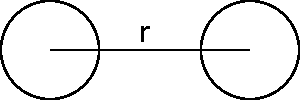
\includegraphics[width=3cm]{radius}\\
		\textbf{Daraus ableitend:}\\
		\(a_1 = \frac{F_1}{m_1}=G\frac{m_2}{r^2} \)\\
		\textbf{und}\\
		\(a_1 + a_2 = G\frac{m_1 + m_2}{r^2}\)\\
		\section{Luftwiderstand}
		\subsection{Konstanten \& andere Werte}
		\(\rho\): Dichte\\
		\(c_w\): Luftwiderstandskoeffizient
		\subsection{Basisformel}
		\( F_w = \frac{1}{2} c_w A  \rho v^2 \)
		\subsection{Maximalgeschwindigkeit}
		\(v_{max} = \sqrt{\frac{2mg}{Ac_w\rho}} \)\\
		In diesem Fall ist \(F_w = F_G\)
	\end{multicols}
\end{document}